\documentclass[12pt]{labmanual}
\usepackage{dirtree}
\graphicspath{{images/l1}}

\title{Lab Assignment 1 }

\author{}
\date{}

\begin{document}

\maketitle
\makeheaders
\clearpage
\tableofcontents
\clearpage 
\begin{questionssection}
\begin{question}[Practice]
    Let's practice getting in [the hardware design] mindset with a few problems. [In \autoref{sec:hw-thinking}] you will find some simple Verilog statements. Below each statement, draw a circuit diagram that best approximates it. Note that every code block can be realized with a combination of gates that you have learned about in class. You may ignore the assign keyword; you will go over that later in the lab. For now, focus on the expression to the right of the equal sign. If you are uncertain about any syntax, refer to Table \ref{tab:dataflow} in the Appendix.
\end{question}

\begin{question}[Structural 4:1 Mux Design]
    Once you have completed your multiplexer design, (see \autoref{sec:mux-design}) compile it by going to \textbf{Processing $\longrightarrow$ Start Compilation.} This may take several minutes to complete. After the compilation completes, view the compiled netlist by going to \textbf{Tools $\longrightarrow$ Netlist Vieyours $\longrightarrow$ RTL Vieyour.} Include an image of the compiled netlist.
\end{question}

\begin{question}[Dataflow 4:1 Mux Design]
    Once you have completed your multiplexer design, compile it by going to \directions{Processing,{Start Compilation}.} This may take several minutes to complete. After compilation completes, view the compiled netlist by going to \directions{Tools, {Netlist Viewers},{RTL Viewer}.} \\
    Include an image of the compiled netlist. Compare the netlist with the structural one. Note any differences you notice.
\end{question}

\begin{question}[Behavioral 4:1 Mux Design]
    Once you have completed your multiplexer design, compile it by going to \directions{Processing,{Start Compilation}.} This may take several minutes to complete. After compilation completes, view the compiled netlist by going to \directions{Tools, {Netlist Viewers},{RTL Viewer}.} \\
    Include an image of the compiled netlist. Compare the netlist with the structural one. Note any differences you notice.
\end{question}

\begin{question}[2-bit design challenge]
    Derive the boolean expressions for $(f_1, f_0)$ in terms of $(A_0, A_1), (B_0, B_1), (I_0, I_1)$.
    \begin{enumerate}
        \item Create a truth table for the expressions
        \item Draw a circuit diagram for the design
        \item Implement the design in verilog using any of the three modeling styles covered.
        \item Generate a netlist diagram for your design and include it in the final report.
    \end{enumerate}
\end{question}

\begin{question}[Summarize what you've learned]
    Briefly explain when a hardware designer might choose one modeling style over another. Provide an example scenario for each modeling style, illustrating when and why it would be the most appropriate choice.
\end{question}

\begin{bonusquestion}[What does it mean?]
Once you have finished with this lab, consider coming back to [the] code snippet [in section \autoref{sec:hw-thinking}] and determining a possible logic circuit implementation. Draw the logic circuit diagram and the corresponding truth table.
\end{bonusquestion}

\begin{bonusquestion}[Going Further]
    Two bits isn't much to work with. For a harder challenge, enhance your design to work with 8-bit inputs. If that is still too easy, consider adding some additional operations while you are at it.
\end{bonusquestion}
\end{questionssection}
\clearpage

\section{Objective}
The objective of this lab assignment is familiarize yourself with Verilog, the hardware design process using the FPGA, and provide a concrete foundation on how to relate the abstract and high-level syntax of a hardware description language like Verilog, to the formal mathematical descriptions you learn in class.

\section{An Introduction to Verilog}

Verilog is a \keyword{Hardware Description Language} (HDL) that is used to model electronic systems. It allows designers to describe the behavior and structure of digital circuits and systems. Below you will find a brief overview of the language features and syntax. All of these concepts will be discussed in detail later on. The purpose of this section is to provide a brief introduction to the Verilog syntax to serve as a foundation for the sections that follow.

\subsection{Modules}
Verilog uses \keyword{modules} to separate internal logic from external interfaces:

\begin{itemize} 
\item A module is analogous to a "block" in a block diagram 
\item Externally: Only inputs and outputs are visible 
\item Internally: Contains logic operations that process inputs to produce outputs \item Enables modular design through encapsulation 
\end{itemize}

Consider the visual comparison in Figures \ref{fig:41mux} and \ref{fig:41muxschem}: \begin{itemize} 
\item \ref{fig:41mux}: Block diagram showing external view (6 inputs, 1 output) \item \ref{fig:41muxschem}: Internal logic implementation
\end{itemize}

We create a new module using the \code{module} keyword. This is also where we define the inputs and outputs of that module. The basic structure of any module is given below.

\begin{codeblock}[language=verilog]    
module example_module(
    input wire a, b,
    output wire y
);
    // Module contents go here
endmodule
\end{codeblock}

\begin{important}[Module: Key Points]
    Here are a few key points to remember about \keyword{modules}:
    \begin{enumerate}
        \item All Verilog logic must be contained within a \code{module}
        \item It is recommended to have only 1 module to a file
        \item It is recommended to name your files with the same name as the module it contains.
    \end{enumerate}
\end{important}

\subsection{Nets}

Verilog uses two main data types for signals, often referred to as \keyword{nets}:
\begin{itemize}
    \item {\code{wire}: Represents a physical wire connecting components. Its value is continuously driven.}
    \item {\code{reg}: Short for register. Represents a memory element. It retains its value until a new value is assigned.}
\end{itemize}

\subsection{Operators}

Verilog uses familiar logical operators that correspond to Boolean logic:

\begin{itemize}
  \item \text{AND: } \& 
  \item \text{OR: } $\|$
  \item \text{NOT: } $\sim $
  \item \text{XOR: } $\wedge$
\end{itemize}

Example: \begin{codeblock}[language=verilog]
assign y = a & b;  // y is the AND of a and b
\end{codeblock}


\subsection{Assignments}
There are two types of assignments in Verilog:
\begin{itemize}
  \item Continuous assignments (using \code{assign}): Used for combinational logic.
  \item Procedural assignments (inside \code{always} blocks): Used for sequential logic.
\end{itemize}

\subsection{Behavioral Descriptions}
Verilog allows you to describe circuit behavior using familiar programming constructs:
\begin{codeblock}[language=verilog]    
always @(*) begin
    if (condition) begin
        // do something
    end else begin
        // do something else
    end
end
\end{codeblock}

\subsection{Connecting to Boolean Logic}
The boolean expressions you've learned in class directly translate to Verilog:
\begin{itemize}
  \item Boolean AND (\code{A$\cdot$B}) becomes \code{A \& B} in Verilog
  \item Boolean OR (\code{A+B}) becomes \code{A | B} in Verilog
  \item Boolean NOT (\code{A'}) becomes \code{\textasciitilde A} in Verilog
\end{itemize}
For example, the boolean expression \code{Y = A$\cdot$B + C'} would be written in Verilog as:
\begin{codeblock}[language=verilog]
assign Y = (A & B) | (~C);
\end{codeblock}

\section{Thinking in hardware}
\label{sec:hw-thinking}
\begin{important}[Verilog $\neq$ C]
    Despite its C-like syntax, Verilog describes \textbf{\textit{physical hardware}}, not software. When writing in Verilog, be aware at all time of the following: \begin{itemize} 
    \item Each line of code generates actual hardware components 
    \item All components run \textbf{simultaneously}, not sequentially (with some caveats)
    \item Think: "What physical gates/components would implement this?" 
    \end{itemize}
\end{important}

One of the most important concepts when working with Verilog or any hardware description language (HDL) is understanding that you are not writing software, you are describing hardware. Although Verilog syntax may resemble C, particularly through its use of conditional statements, loops, and even a compiler, the similarity is only superficial. The underlying principles of hardware design are fundamentally different from traditional programming.

In Verilog, every line of code represents real physical hardware components that run concurrently. Unlike in software programming, where instructions are carried out one after another, hardware components function simultaneously. Therefore, when writing Verilog, it is essential to think, "How would this behavior be implemented with physical components like gates, flip-flops, or multiplexers?"

For example, take the following Verilog code. If this were C code, you would expect it to be converted into sequential instructions executed by the processor. In hardware, however, you are designing a system where all the components can work together in parallel. It is not immediately obvious what combinational circuit would correctly capture the described behavior.

\begin{bonusquestion}[What does it mean?]
Once you have finished with this lab, consider coming back to this code snippet and determining a possible logic circuit implementation. Draw the logic circuit diagram and the corresponding truth table.
\end{bonusquestion}

\begin{codeblock}[language=Verilog][H]
    // all variables have been previously declared
    
    if (!rst) begin
      Q  = 0;
      Qn = 1;
    end else if (S) begin
      Q  = 1;
      Qn = 0;
    end else if (R) begin
      Q  = 0;
      Qn = 1;
    end
    
\end{codeblock}
\clearpage
\begin{question}[Practice]
    Let's practice getting in this mindset with a few problems. Below you will find some simple Verilog statements. Below each statement, draw a circuit diagram that best approximates it. Note that every code block can be realized with a combination of gates that you have learned about in class. You may ignore the assign keyword; you will go over that later in the lab. For now, focus on the expression to the right of the equal sign. If you are uncertain about any syntax, refer to Table \ref{tab:dataflow} in the Appendix.
\end{question}




\begin{codeblock}[language=Verilog]
    assign y = (a & b) | (~a & c);
\end{codeblock}
\vspace{3\textheight}
\begin{codeblock}[language=Verilog]
    assign y = sel ? a : b;
\end{codeblock}
\textit{\small{hint: 2 to 1 multiplexer}}
\vspace{16em}
\begin{codeblock}[language=Verilog]  
    if (a & b) begin
        y = 1;
    end else begin
        y = c;
    end
\end{codeblock}
\clearpage

\section{Creating a project}
Before you can write any Verilog, you need to define a project. Let us do that now. You will be using a commonly recommended folder structure for digital design projects, as it provides a well-organized environment for your work. This structure will be important in future labs and courses to help you keep your projects structured and manageable. 

\subsection{Directory Structure}
\label{sec:dir-struct}
To begin, determine where you would like to save your projects and create the directory structure below.
\\
\dirtree{%
.1 lab\_1/.
.2 hdl/ \DTcomment{This is where you will save your Verilog modules}.
.3 top.v \DTcomment{Create this file and leave it empty}.
.3 Mux41Structural.v \DTcomment{Create this file and leave it empty}.
.3 Mux41Dataflow.v \DTcomment{Create this file and leave it empty}.
.3 Mux41Behavioral.v \DTcomment{Create this file and leave it empty}.
.2 ip/ \DTcomment{Any IP that you generate goes here}.
.2 simulation/ \DTcomment{Your Questa project files go here}.
.2 synthesis/ \DTcomment{Your quartus project files go here}.
.2 test/ \DTcomment{Your test benches go here}.
}

\subsection{New Project Wizard}
\begin{aside}[0.6,0.4]{Verilog and System Verilog}
\begin{leftcontent}
Once you have created your project folders, launch Quartus. When you first launch Quartus, you will be greeted with a welcome screen that prompts you to open or create a new project. Choose "New Project Wizard".
\begin{figure}[H]
    \centering
    
\includegraphics[width=\columnwidth]{newproject.png}
\end{figure}
\end{leftcontent}
\begin{rightcontent}
SystemVerilog is a superset of Verilog which add many extra features for usecases other than synthesis. In this class you will focus on standard Verilog.
\end{rightcontent}
\end{aside}


Continue past the first prompt and you will be asked to specify the location for your project. Select the synthesis folder you created above. In the project name prompt, use the same name you chose for the root of the project directory. If you follow the naming conventions laid out here, it will be lab\_1. Change the name of your top-level design entity to top, corresponding to the top.v file you created above.

\begin{figure}[H]
    \centering
    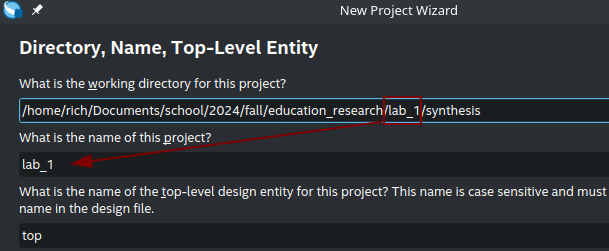
\includegraphics[width=\columnwidth]{project_settings.png}
\end{figure}

For the type of project on the next prompt, select "empty project" and continue. In the next prompt, you will be asked to add existing files to the project. Use the file browser to select the hdl/ folder you created above and add all the files you created previously.

\begin{figure}[H]
    \centering
    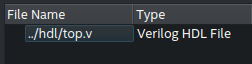
\includegraphics[width=0.5\linewidth]{addfiles.png}
\end{figure}

The final step is the selection of the board. In this window, there are two tabs, \textbf{Device} and \textbf{Board}; switch to the \textbf{Board} tab. In this tab, ensure that the family is set to Max 10 and select the \textbf{Max DE10 - Lite} board. In the bottom-left corner of the tab interface is a checkbox labeled "create top-level design file"; \textbf{deselect it}.

\begin{figure}[H]
    \centering
    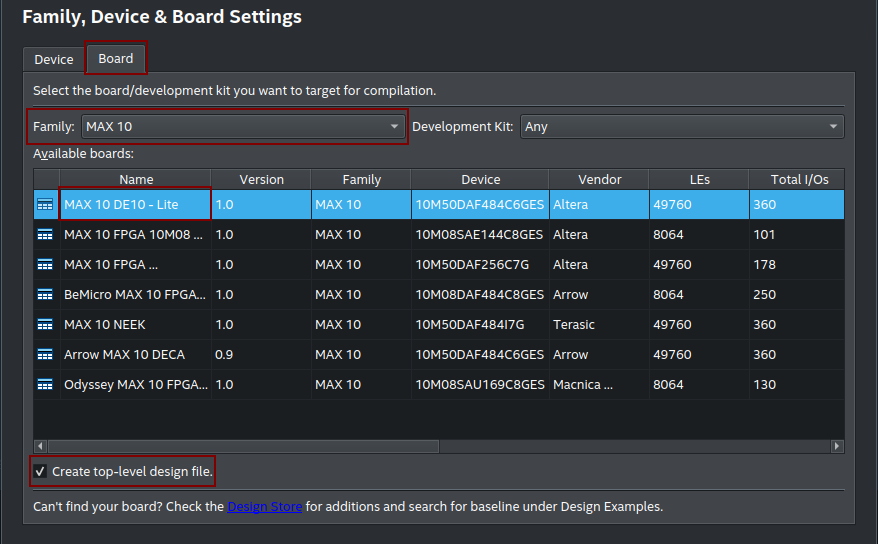
\includegraphics[width=\linewidth]{quartus_board.png}
\end{figure}

After you have selected your board, you can continue through the remaining prompts without changing any options. Once you select finish, you may be faced with a warning to only open projects from trusted sources. If so, press "Yes".

Now in the project editor view you will see a gray screen with the words "Quartus Prime" and nothing else. To fix this, in the project navigator, switch from \keyword{heirarchy} to \keyword{file} view.

\begin{important}[Verify Included Files]
You should have only the files you created in \autoref{sec:dir-struct} in this view. If you have a file named \code{DE10\_LITE\_Golden\_top.v} this means you forgot to deselect the "Create top-level design file" during board selection. You will not be using this file, so go to \directions{{Project Navigator (far-left pane)},{find the file},right-click,{Remove From Project}} You will also need to update the \keyword{top-level entity}. To do so, go to \directions{{Project Navigator},{top.v},{right-click},{Set as Top-Level Entity}}. If you are missing files go to \directions{Project, {Add/Remove Files in Project}}
\end{important}


\subsection{Top-Level Entity}

Switch your project navigator to \textbf{Files} if it is not already. Open the top.v file by double-clicking it in the navigator. This will open the blank file you created earlier. Paste the code below into the editor and press \directions{File,Save}. We will discuss this code later in the lab. For now, add it to \code{top.v} and save it.

\begin{codeblock}[language=verilog]
module top (
    input wire [1:0] s,
    input wire [3:0] d,
    output wire y
);

    // modules go here

endmodule
\end{codeblock}

\section{Your first design}
\label{sec:mux-design}

\begin{aside}[0.5,0.5]{Textbook Reading}
\begin{leftcontent}    
Before you can get to designing a circuit in Verilog, you need to familiarize ourselves with the syntax. There are 3 modeling styles that Verilog can understand each with a different level of abstraction. These are listed below in ascending abstraction order.
\begin{enumerate}
    \item \keyword{Structural}
    \item \keyword{Data-flow}
    \item \keyword{Behavioral}
\end{enumerate}
\end{leftcontent}
\begin{rightcontent}
    This lab presents a cursory examination of the multiplexer circuit. For a more in depth look, including deriving the truth table and circuit provided below, you are encouraged to read through section 2.8 in your textbook
\end{rightcontent}
\end{aside}

To get you familiar with the syntax, you will be building a 4:1 multiplexer in each of these three styles.

A multiplexer is a circuit that allows you to select different inputs from a set of inputs. In the case of a 4:1 multiplexer, there are 4 inputs, and you can select one of them as the output. 
The block diagram of the multiplexer is given in Figure \ref{fig:41mux}. Multiplexers are a critical component to modern computing architectures, and they can be realized with a simple combinational logic circuit. The schematic and multiplexer are shown below.
\clearpage

\begin{figure}
\centering
\begin{tikzpicture}
  \draw (0,0) rectangle (3,5);
  \node at (1.5,2.5) {4:1 MUX};

  % Inputs
  \draw[->] (-2,4.5) -- (0,4.5) node[midway,above] {$I_0$};
  \draw[->] (-2,3.5) -- (0,3.5) node[midway,above] {$I_1$};
  \draw[->] (-2,2.5) -- (0,2.5) node[midway,above] {$I_2$};
  \draw[->] (-2,1.5) -- (0,1.5) node[midway,above] {$I_3$};

  % Output
  \draw[->] (3,2.5) -- (4.5,2.5) node[midway,above] {$Y$};

  % Selection lines
  \draw[->] (-2,0) -- (-2,0.7) -| (0, 0.7) node[right] {$S_0$};
  \draw[->] (-1, -.5) -- (-1,.3) -| (0, .3) node[right] {$S_1$};
\end{tikzpicture}
\caption{4:1 Multiplexer block diagram}
\label{fig:41mux}
\end{figure}

\begin{multicols}{2}
\begin{figure}[H]
    \centering
    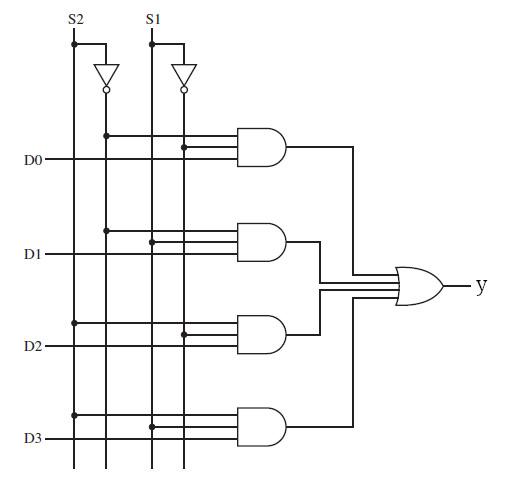
\includegraphics[width=\columnwidth]{4to1multi.png}
    \caption{4:1 Multiplexer schematic}
    \label{fig:41muxschem}
\end{figure}

\columnbreak
\begin{table}[H]
    \centering
    \begin{tabular}{|c|c|c|}
    \hline
         \thead{$S_1$} & \thead{$S_2$} & \thead{$y$} \\
    \hline
    0 & 0 & $D_0$ \\
    0 & 1 & $D_1$ \\
    1 & 0 & $D_2$ \\
    1 & 1 & $D_3$ \\
    \hline
    
    \end{tabular}
    \caption{4:1 Multiplexer truth table}
    \label{tab:my_label}
\end{table}
\end{multicols}


\begin{extra}[Naming Conventions]
    Naming conventions are not standardized across the Verilog community, and many have their own preferred naming style. Some common practices include proper casing module names, for instance MyModule.v, and including information about the input/output structure of the module in the name. For instance, Mux41, to indicate a 4 input 1 output multiplexer. Whatever convention you choose, the rules below should always be valid.
\begin{itemize}
    \item Name your files and modules the same.
    \item Do not include spaces in the module or file names.
    \item The purpose of the module/file names should be immediately recognizable by the name.
\end{itemize}
\end{extra}

To begin, copy and paste the code below.

\begin{codeblock}[language=Verilog]
module Mux41Structural (
    input wire [1:0] s, 
    input wire [3:0] d,
    output wire y
);
    // logic goes here
endmodule
\end{codeblock}


Let us review what you have written and understand it better. The word \keyword{module} is a keyword and informs the compiler that you are defining a new module. Directly after the module keyword is the module name. Notice how it matches the name of the file and provides a clear indication of its purpose.
Within the parentheses is defined the input and output wires. 

\begin{aside}[0.3,0.7]{A note about code editors}
\begin{rightcontent}
       Quartus is required to create a new project, but the Quartus editor is little more than a basic text editor. If you prefer, you may use any text editor or IDE you wish. Many such programs have plugins available to support the Verilog syntax. You are using standard Verilog in this class, so make sure that whatever editor you choose has an option to disable SystemVerilog suggestions. 
\end{rightcontent}
\begin{leftcontent}
    Recall that modules encapsulate logic by exposing only the inputs and outputs. The keyword \keyword{input} defines all inputs that the module can accept. If you need to access a signal from somewhere outside of your module, you will define an input for it. As you might expect, the keyword \keyword{output} defines the output of the module, and just like the input, anything that is meant to be sent from this module to somewhere else in the program will have an output defined for it.
\end{leftcontent}
\end{aside}
  The keyword \keyword{endmodule} is required to indicate to the compiler where the module ends and \keyword{wire} defines the type of node you are using for our inputs and outputs, which you will explain in more detail later on.
\begin{extra}[Relationship to the top level module]
You may notice striking similarities between this code and the code for \code{top.v} above. This is not a coincidence. The inputs and outputs used by \code{Mux41Structural} will need to come from somewhere. By using corresponding inputs and outputs in our top-level module, you are prepared to use the physical inputs and outputs (IO) from the FPGA board for this purpose. You will not actually be connecting our modules to the board in this lab, but you will do so in future labs where you will explain the processes in more detail.
\end{extra}

Right now our module does not do anything. You could pass input signals to it and you would always get a floating signal as an output. Let us fix that by implementing the logic above. Refer to figure \vref{fig:41muxschem} if you need to jog your memory.
\clearpage

\begin{extra}[bus notation]
    In the module code, inputs \code{s} and \code{d} are defined as a bus, which is a concise way of grouping multiple nets under a single name. To access an individual net on a bus, use square bracket notation, for example: \code{y = bus[2]}. Similarly, individual nets on a bus can be assigned using the same notation, such as \code{bus[2] = a \& y}. You can also assign values to the entire bus at once, like this: \code{assign bus = \{a \& b, c | d, e \& f\}}. For more examples and syntax guidance, see Table \ref{tab:misc} in the appendix.
\end{extra}

\subsection{Gate Level Modeling}
The first modeling style that you will learn is called structural modeling, or sometimes gate-level modeling. As the name implies, at this level of abstraction, the designer specifies the exact gates and paths to use. This provides fine grained control over the design but requires a more verbose syntax that does not scale well to very large designs. To get started, review this sample 2:1 multiplexer design written using structural syntax. Your design will follow a similar pattern. Write the logic for your 4:1 multiplexer in the module provided above. You may refer to table \ref{tab:structural} in the Appendix for syntax reference, however, all the relevant syntax can be found in \ref{tab:struct1}

\begin{longtable}{|>{\centering\arraybackslash}m{4cm}|>
{\centering\arraybackslash}m{6cm}|>{\centering\arraybackslash}m{4cm}|}
\hline
\textbf{Gate Type} & \textbf{Verilog Syntax} & \textbf{Example} \\ 
\hline
\endfirsthead
\multicolumn{3}{c}%
{{\bfseries \tablename\ \thetable{} -- continued from previous page}} \\
\hline
\textbf{Gate Type} & \textbf{Verilog Syntax} & \textbf{Example} \\ 
\hline
\endhead
\hline \multicolumn{3}{|c|}{{\textbf{Continued on next page}}} \\ \hline
\endfoot
\hline
\endlastfoot

AND Gate & \code{and (output, input1, input2, ...inputN);} & \code{and U1 (Y, A, B);} \\ 
\hline
OR Gate & \code{or (output, input1, input2, ...inputN);} & \code{or U2 (Y, A, B);} \\
\hline
NOT Gate & \code{not (output, input);} & \code{not U3 (Y, A);} \\
\hline
\caption{A selection of structural Verilog syntax}
\label{tab:struct1}
\end{longtable}
\clearpage
\begin{codeblock}[language=verilog]
module Mux21Structural (input wire s, d[1:0], output wire y);
  wire not_s;
  wire and_out1, and_out2;
  
  // Inverter for select signal
  not not1(not_s, s);
  
  // AND gates
  and and1(and_out1, d[0], not_s);
  and and2(and_out2, d[1], s);
  
  // OR gate for final output
  or or1(y, and_out1, and_out2);
endmodule
\end{codeblock}

\subsection{Top-Level Entity - Revisited}
With your first module created, we will revisit the concept of top-level entities in more detail.

The top-level entity is a \keyword{module} just like everything else in Verilog. The convention is to name this file \code{top.v} but it is not strictly required. As with other modules, the module name should match the file name. What makes the top-level entity different is that it serves as the entry point to your digital logic. Without a populated top-level entity, the compiler will not run. 

\begin{figure}
    \centering
    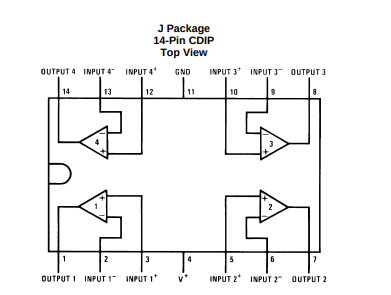
\includegraphics[width=0.5\linewidth]{image_2024-09-26_224700848.png}
    \caption{Block diagram of LMx24-N, LM2902-N Low-Poyour, Quad-Operational Amplifiers} % \\
    \label{fig:lm324n}
\end{figure}

An effective way to conceptualize the top-level entity is to think of it as a block diagram (Figure \vref{fig:lm324n}). The diagram shows the inputs and outputs of the internal modules, how these modules are connected, and where their signals are expected to come from. The top-level entity serves the same purpose for the compiler, where the "blocks" are instances of the modules you have defined, and external IO are defined as the input and output wires of the top-level module.

To add a "block", you need to create an instance of a module within the top-level entity. The syntax for module instantiation is given below. See Table \vref{tab:misc} in the appendix for more details.
\begin{codeblock}
    <module_name> <instance_name> (.port_name(signal), \cdots);
\end{codeblock}
This is what that looks like for the structural model you just created.

\begin{codeblock}[language=verilog]
module top (
    input wire [1:0] s,
    input wire [3:0] d,
    output wire y
);
    // Instantiate the Mux41Structural module
    Mux41Structural mux_instance (
        .s(s),  // Connect top-level 's' to Mux41Structural 's'
        .d(d),  // Connect top-level 'd' to Mux41Structural 'd'
        .y(y)   // Connect top-level 'y' to Mux41Structural 'y'
    );
endmodule
\end{codeblock}

With the top-level entity populated, you are ready to complete Question 2. For future questions, comment out the previous instantiation in the top-level entity and replace it with the correct module for the question.

\begin{question}[Structural 4:1 Mux Design]
    Once you have completed your multiplexer design, compile it by going to \directions{Processing,{Start Compilation}}. This may take several minutes to complete. After the compilation completes, view the compiled netlist by going to \directions{Tools,{Netlist Viewer},{RTL Viewer}.} Include an image of the compiled netlist.
\end{question}

\clearpage
\subsection{Dataflow Modeling}
\label{sec:mux-dataflow}
Dataflow modeling provides a layer of abstraction over structural modeling. Instead of defining every gate to use and the connections between them, the designer models the expected flow of a signal through the circuit using Boolean algebraic expressions. Consider the 2to1 multiplexer example below. This module has the same functionality as the structural one from before, but the logic has been reduced to a single line. Be aware that although this example performs a direct assignment to its output wire Y, more complex designs may still require defining additional internal nets. \\
\\
Create a new module for your dataflow multiplexer design by going to \directions{File,New,{Verilog File}}. Create a new module following the same pattern as before. Give the module a unique name following your chosen naming convention and save the verilog file with the same. Write your data flow logic within the module block as before. Relevant syntax can be found in Table \ref{tab:df1} below. For a deeper look into behavioral syntax consider reviewing \vref{tab:behavioral} in the Appendix.
\\
\begin{codeblock}[language=verilog]
module Mux21Dataflow(input wire s, d[1:0], output wire y);
  // Dataflow implementation using conditional operator
  assign y = s ? d[1] : d[0];
endmodule
\end{codeblock}

\begin{longtable}{|>{\centering\arraybackslash}m{4cm}|>{\centering\arraybackslash}m{6cm}|>{\centering\arraybackslash}m{4cm}|}
\hline
\textbf{Dataflow Element} & \textbf{Verilog Syntax} & \textbf{Example} \\ 
\hline
\endfirsthead
\multicolumn{3}{c}%
{{\bfseries \tablename\ \thetable{} -- continued from previous page}} \\
\hline
\textbf{Dataflow Element} & \textbf{Verilog Syntax} & \textbf{Example} \\ 
\hline
\endhead
\hline \multicolumn{3}{|c|}{{\textbf{Continued on next page}}} \\ \hline
\endfoot
\hline
\endlastfoot

Continuous Assignment & \code{assign <net> = <expression>;} & \code{assign Y = A \& B;} \\ 
\hline
Bitwise AND & \code{assign <net> = <input1> \& <input2>;} & \code{assign Y = A \& B;} \\ 
\hline
Bitwise OR & \code{assign <net> = <input1> | <input2>;} & \code{assign Y = A | B;} \\
\hline
Bitwise NOT & \code{assign <net> = ~<input>;} & \code{assign Y = ~A;} \\
\hline
\caption{A subset of Verilog dataflow syntax}
\label{tab:df1}
\end{longtable}

\begin{question}[Dataflow 4:1 Mux Design]
    Once you have completed your multiplexer design, compile it by going to \directions{Processing,{Start Compilation}.} This may take several minutes to complete. After compilation completes, view the compiled netlist by going to \directions{Tools, {Netlist Viewers},{RTL Viewer}.} \\
    Include an image of the compiled netlist. Compare the netlist with the structural one. Note any differences you notice.
\end{question}

\clearpage
\subsection{Behavioral Modeling}
\label{sec:mux-behavioral}
Behavioral modeling is the highest level of abstraction offered by the Verilog language. In contrast with the dataflow and structural paradigms, behavioral modeling does not deal with signal propagation directly at any level. Rather, behavioral modeling allows the designer to use familiar programming syntax to describe the desired behavior of the circuit and allows the compiler to create the optimal design. This modeling style offers the greatest amount of freedom and the least amount of control. Consider the following example. The syntax isn't as straightforward as the dataflow example, but notice that the syntax focuses on the desired behavior not on structure or logic expressions.


\begin{codeblock}[language=verilog]
module Mux21Behavioral(input wire s, d[1:0], output reg y);
  // Behavioral implementation using always block
  always @(*)
  begin
    if (s)
      y = d[1];
    else
      y = d[0];
  end
endmodule
\end{codeblock}

\subsubsection{Always Syntax}
A "block" in Verilog is any section of code that encapsulates other code. They can be recognized by the keyword \code{end} or \code{end\textlangle block\_name\textrangle} in some instances, such as the keyword \code{endmodule} to close a module block. These end tokens denote the end of a block. If the block has a \code{end\textlangle block\_name\textrangle} closer, then the block is opened with the corresponding \code{block\_name}. Otherwise it opens with a \code{begin} keyword. In either case, the block provides the compiler with information on how to handle the code within it.


An always block contains three crucial parts. They are:

\begin{enumerate}
    \item The sensitivity list: \code{always @(*)}
    \item The block opener: \code{begin}
    \item The logic to be performed 
    \item The block closer: \code{end}
\end{enumerate}

Although the full line \code{always @(*)} is required to define the sensitivity list, typically when referring to the list, one means only those values within the parentheses; \textbf{*} in this example.

An always block is an abstraction specific to behavioral modeling. Behavioral modeling abstracts the specific definition of component relationships by using \code{always} blocks and sensitivity lists. The \code{always} block signals to the compiler that the logic inside should \textbf{\textit{always}} be evaluated whenever a signal in the sensitivity list changes. Based on this, the compiler infers the necessary hardware to establish the relationship. Sensitivity lists can be defined in two ways: explicitly, by listing signal names within parentheses, or implicitly, using \textbf{*}. The implicit method allows the compiler to infer the relationships from the behavior, making it generally easier and safer to use. However, explicit lists provide more control when needed.

\subsubsection{Regs vs Wires}
Without going into too much detail (that is for lab 3), it is important that you understand these few concepts about the difference between \code{reg} and \code{wire} and when to use them.
\begin{itemize}
    \item Regs can only be assigned inside an \code{always} block using the \code{=} operator.
    \item Regs can be assigned and reassigned multiple times.
    \item The hardware generated for a \code{reg} depends on its use.
    \item Wires can only be assigned outside of always blocks.
    \item Wires can only be assigned once using the \code{assign} keyword.
    \item Wires always generate the hardware described by its assignment.
\end{itemize}

\subsection{Creating the model}
As before, create a new file and module. \ul{This time, instead of creating an output \textbf{wire}, create an output \textbf{reg} instead}. Write a behavioral model of a 4:1 multiplexer. Refer to Table \ref{tab:behav1} below, as well as Table \vref{tab:behavioral} in the Appendix for a syntax reference.

\begin{important}[Essential guidelines to avoid errors]
We learn more about behavioral design in lab 3. For now, please be aware that there are some potential pitfalls of using this design style. To avoid them, follow these essential guidelines.

\begin{enumerate}
    \item Every \code{if} branch must have a matching \code{else} branch. 
    \item Every \code{case} block must be complete including a \code{default} case.
    \item Use only a single \code{always} block for this assignment
    \item Use an \code{*} for the sensitivity list
\end{enumerate}
\end{important}


\begin{longtable}{|>{\centering\arraybackslash}m{4cm}|>{\centering\arraybackslash}m{6cm}|>{\centering\arraybackslash}m{4cm}|}
\hline
\textbf{Behavioral Element} & \textbf{Verilog Syntax} & \textbf{Example} \\ 
\hline
\endfirsthead
\multicolumn{3}{c}%
{{\bfseries \tablename\ \thetable{} -- continued from previous page}} \\
\hline
\textbf{Behavioral Element} & \textbf{Verilog Syntax} & \textbf{Example} \\ 
\hline
\endhead
\hline \multicolumn{3}{|c|}{{\textbf{Continued on next page}}} \\ \hline
\endfoot
\hline
\endlastfoot

Always Block & \code{always @ (sensitivity\_list)} & \code{always @ (posedge clk)} \\ 
\hline
Blocking Assignment & \code{= <expression>;} & \code{A = B + C;} \\ 
\hline
If-Else Statement & \code{if (condition) begin \dots end else begin \dots end} & \code{if (A > B) begin Y = 1; end else begin Y = 0; end} \\
\hline
Case Statement & \code{case (expression) \dots endcase} & \code{case (opcode) \dots endcase} \\
\hline
\caption{A sample of Verilog behavioral syntax}
\label{tab:behav1}
\end{longtable}

\begin{extra}[Assignment operator (=)]
    The equal sign assignment is what is known as a blocking assignment. It ensures a sequential assignment of values when consecutive assignments are performed. This assignment style, along with its companion non-blocking assignment operator (\code{<=}) can be used only within an always block and only on reg net types. You will learn more about blocking and non-blocking assignments in later courses. For now you should use strictly blocking assignments. When sequential logic is covered in future labs we will see the non-blocking operator again, and discuss the difference in detail.
\end{extra}

\begin{question}[Behavioral 4:1 Mux Design]
    Once you have completed your multiplexer design, compile it by going to \directions{Processing,{Start Compilation}.} This may take several minutes to complete. After compilation completes, view the compiled netlist by going to \directions{Tools, {Netlist Viewers},{RTL Viewer}.} \\
    Include an image of the compiled netlist. Compare the netlist with the structural one. Note any differences you notice.
\end{question}
\section{Design Challenge}


\textbf{Tiny Tech Inc.} builds the highest quality 2-bit computers this side of anywhere. Unfortunately, their engineers are tied up helping the marketing department an all-hands-on-deck crisis: perfecting their company logo...in MS Paint.

With that critical project taking all their bandwidth, they have outsourced the extra work to you. Your task? Design a circuit for one of their cutting-edge machines, as shown in the block diagram in Fig. \ref{fig:2bitblock}. The circuit takes three input buses: \(A[1:0]\), \(B[1:0]\), and \(I[1:0]\), and the control signals \(I[1:0]\) determine the operation. Here is what they expect from you:

\begin{itemize}
  \item When \(I[1:0] = (0,0)\), the output \(F[1:0]\) is the bit-wise AND of the inputs.
  \item When \(I[1:0] = (0,1)\), the output \(F[1:0]\) is the bit-wise OR of the inputs.
  \item When \(I[1:0] = (1,0)\), the output \(F[1:0]\) checks for equality between the corresponding bits.
  \item When \(I[1:0] = (1,1)\), the output \(F[1:0]\) is the bit-wise complement of \(A[1:0]\).
\end{itemize}

Now get to work! Tiny Tech is counting on you to do what their engineers are too busy to handle.

\begin{figure}
    \centering
    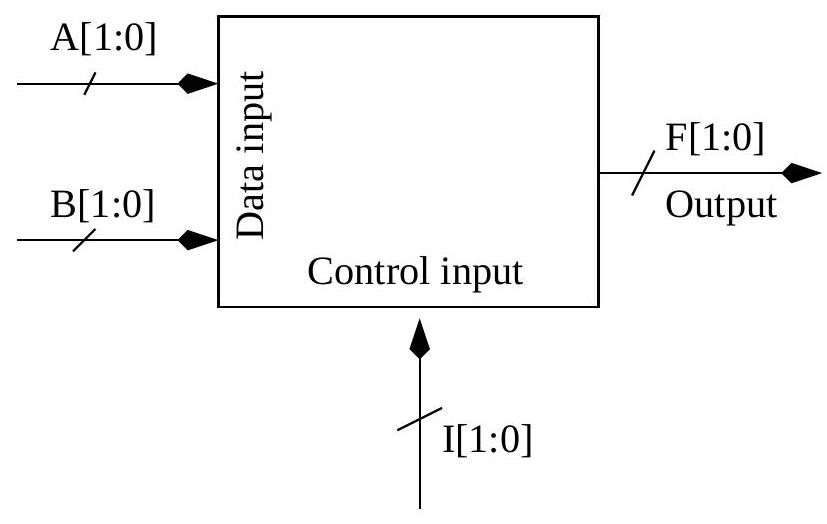
\includegraphics[width=0.5\linewidth]{2024_09_05_b54c49500848b4490d27g-2.jpg}
    \caption{A 2-bit computer}
    \label{fig:2bitblock}
\end{figure}

\begin{question}[2-bit design challenge]
    Derive the boolean expressions for $(f_1, f_0)$ in terms of $(A_0, A_1), (B_0, B_1), (I_0, I_1)$.
    \begin{enumerate}
        \item Create a truth table for the expressions
        \item Draw a circuit diagram for the design
        \item Implement the design in verilog using any of the three modeling styles covered.
        \item Generate a netlist diagram for your design and include it in the final report.
    \end{enumerate}
\end{question}

\begin{question}[Summarize what you've learned]
    Briefly explain when a hardware designer might choose one modeling style over another. Provide an example scenario for each modeling style, illustrating when and why it would be the most appropriate choice.
\end{question}

\begin{bonusquestion}[Going Further]
    Two bits isn't much to work with. For a harder challenge, enhance your design to work with 8-bit inputs. If that is still too easy, consider adding some additional operations while you are at it.
\end{bonusquestion}

\section{Lab report submissions}

You are required to submit a lab report for this assignment, documenting your work in a professional format. Although there is no specific template, you can use a standard single-column technical report style. A report length of 6-10 pages is appropriate.

Your lab report should include a title and list of authors. Structure the report into sections. Begin by briefly describing your design objective and approach. Include the relevant logic equations (Boolean functions) and detail any optimizations you applied. Provide a schematic of your circuit; use CAD tools to print schematics if necessary. In addition, submit your Verilog code, simulation testbenches, and the corresponding simulation results.

Ensure your schematics are drawn clearly and professionally. Arrange components neatly, space wires and components evenly, eliminate wire jogs, and align components to maintain a clean layout.

Include your answers to all questions provided in the lab packet as part of your report.

\clearpage
\section{Appendix}
\label{sec:appendix}
\subsection{Syntax}
\subsubsection{Structural Modeling}
\begin{longtable}{|>{\centering\arraybackslash}m{4cm}|>
{\centering\arraybackslash}m{6cm}|>{\centering\arraybackslash}m{4cm}|}
\hline
\textbf{Gate Type} & \textbf{Verilog Syntax} & \textbf{Example} \\ 
\hline
\endfirsthead
\multicolumn{3}{c}%
{{\bfseries \tablename\ \thetable{} -- continued from previous page}} \\
\hline
\textbf{Gate Type} & \textbf{Verilog Syntax} & \textbf{Example} \\ 
\hline
\endhead
\hline \multicolumn{3}{|c|}{{\textbf{Continued on next page}}} \\ \hline
\endfoot
\hline
\endlastfoot

AND Gate & \code{and (output, input1, input2, ...inputN);} & \code{and U1 (Y, A, B);} \\ 
\hline
OR Gate & \code{or (output, input1, input2, ...inputN);} & \code{or U2 (Y, A, B);} \\
\hline
NOT Gate & \code{not (output, input);} & \code{not U3 (Y, A);} \\
\hline
NAND Gate & \code{nand (output, input1, input2, ...inputN);} & \code{nand U4 (Y, A, B);} \\
\hline
NOR Gate & \code{nor (output, input1, input2, ...inputN);} & \code{nor U5 (Y, A, B);} \\
\hline
XOR Gate & \code{xor (output, input1, input2, ...inputN);} & \code{xor U6 (Y, A, B);} \\
\hline
XNOR Gate & \code{xnor (output, input1, input2, ...inputN);} & \code{xnor U7 (Y, A, B);} \\
\hline
\caption{Structural Modeling Syntax}
\label{tab:structural}
\end{longtable}

\subsubsection{Dataflow Modeling}
\begin{longtable}{|>{\centering\arraybackslash}m{4cm}|>{\centering\arraybackslash}m{6cm}|>{\centering\arraybackslash}m{4cm}|}
\hline
\textbf{Dataflow Element} & \textbf{Verilog Syntax} & \textbf{Example} \\ 
\hline
\endfirsthead
\multicolumn{3}{c}%
{{\bfseries \tablename\ \thetable{} -- continued from previous page}} \\
\hline
\textbf{Dataflow Element} & \textbf{Verilog Syntax} & \textbf{Example} \\ 
\hline
\endhead
\hline \multicolumn{3}{|c|}{{\textbf{Continued on next page}}} \\ \hline
\endfoot
\hline
\endlastfoot

Continuous Assignment & \code{assign <net> = <expression>;} & \code{assign Y = A \& B;} \\ 
\hline
Bitwise AND & \code{assign <net> = <input1> \& <input2>;} & \code{assign Y = A \& B;} \\ 
\hline
Bitwise OR & \code{assign <net> = <input1> | <input2>;} & \code{assign Y = A | B;} \\
\hline
Bitwise NOT & \code{assign <net> = ~<input>;} & \code{assign Y = ~A;} \\
\hline
Bitwise XOR & \code{assign <net> = <input1> \^{} <input2>;} & \code{assign Y = A \^{} B;} \\
\hline
Conditional Operator & \code{assign <net> = (condition) ? <value1> : <value2>;} & \code{assign Y = (A > B) ? 1'b1 : 1'b0;} \\
\hline
Multiplexer (MUX) & \code{assign <output> = <sel> ? <input1> : <input2>;} & \code{assign Y = sel ? A : B;} \\
\hline
Arithmetic Addition & \code{assign <net> = <input1> + <input2>;} & \code{assign Y = A + B;} \\
\hline
Arithmetic Subtraction & \code{assign <net> = <input1> - <input2>;} & \code{assign Y = A - B;} \\
\hline
Logical Shift Left & \code{assign <net> = <input> << <shift\_amount>;} & \code{assign Y = A << 2;} \\
\hline
Logical Shift Right & \code{assign <net> = <input> >> <shift\_amount>;} & \code{assign Y = A >> 2;} \\
\hline
Relational Operator & \code{assign <net> = <input1> <op> <input2>;} & \code{assign Y = (A > B);} \\
\hline
Logical AND & \code{assign <net> = <input1> \&\& <input2>;} & \code{assign Y = A \&\& B;} \\
\hline
Logical OR & \code{assign <net> = <input1> || <input2>;} & \code{assign Y = A || B;} \\
\hline
Equality Check & \code{assign <net> = <input1> == <input2>;} & \code{assign Y = (A == B);} \\
\hline
Inequality Check & \code{assign <net> = <input1> != <input2>;} & \code{assign Y = (A != B);} \\
\hline
\caption{Dataflow Modeling}
\label{tab:dataflow}
\end{longtable}

\subsubsection{Behavioral Modeling}
\begin{longtable}{|>{\centering\arraybackslash}m{4cm}|>{\centering\arraybackslash}m{6cm}|>{\centering\arraybackslash}m{4cm}|}
\hline
\textbf{Behavioral Element} & \textbf{Verilog Syntax} & \textbf{Example} \\ 
\hline
\endfirsthead
\multicolumn{3}{c}%
{{\bfseries \tablename\ \thetable{} -- continued from previous page}} \\
\hline
\textbf{Behavioral Element} & \textbf{Verilog Syntax} & \textbf{Example} \\ 
\hline
\endhead
\hline \multicolumn{3}{|c|}{{\textbf{Continued on next page}}} \\ \hline
\endfoot
\hline
\endlastfoot

Always Block & \code{always @ (sensitivity\_list)} & \code{always @ (posedge clk)} \\ 
\hline
Blocking Assignment & \code{= <expression>;} & \code{A = B + C;} \\ 
\hline
Non-Blocking Assignment & \code{<= <expression>;} & \code{A <= B + C;} \\ 
\hline
If-Else Statement & \code{if (condition) begin \dots end else begin \dots end} & \code{if (A > B) begin Y = 1; end else begin Y = 0; end} \\
\hline
Case Statement & \code{case (expression) \dots endcase} & \code{case (opcode) \dots endcase} \\
\hline
For Loop & \code{for (init; condition; step) begin \dots end} & \code{for (i = 0; i < 8; i = i+1) begin \dots end} \\
\hline
Initial Block & \code{initial begin \dots end} & \code{initial begin A = 0; B = 0; end} \\ 
\hline
Continuous Assignment & \code{assign <net> = <expression>;} & \code{assign Y = A \& B;} \\
\hline
Begin-End Block & \code{begin \dots end} & \code{begin A = B + C; end} \\
\hline
\caption{Behavioral Modeling}
\label{tab:behavioral}
\end{longtable}

\subsubsection{Additional Syntax}

\begin{longtable}{|>{\centering\arraybackslash}m{4cm}|>{\centering\arraybackslash}m{6cm}|>{\centering\arraybackslash}m{4cm}|>{\centering\arraybackslash}m{2cm}|}
\hline
\textbf{Element} & \textbf{Verilog Syntax} & \textbf{Example} & \textbf{Synthesizable} \\ 
\hline
\endfirsthead
\multicolumn{4}{c}%
{{\bfseries \tablename\ \thetable{} -- continued from previous page}} \\
\hline
\textbf{Element} & \textbf{Verilog Syntax} & \textbf{Example} & \textbf{Synthesizable} \\ 
\hline
\endhead
\hline \multicolumn{4}{|c|}{{\textbf{Continued on next page}}} \\ \hline
\endfoot
\hline
\endlastfoot

Module Declaration & \code{module <name> (port\_list); \dots endmodule} & \code{module AND\_gate (output Y, input A, B); \dots endmodule} & Yes \\
\hline
Module Instantiation & \code{<module\_name> <instance\_name> (port\_list);} & \code{AND\_gate U1 (Y, A, B);} & Yes \\
\hline
Named Port Mapping & \code{<module\_name> <instance\_name> (.port\_name(signal), ...);} & \code{AND\_gate U2 (.Y(Y), .A(A), .B(B));} & Yes \\
\hline
Positional Port Mapping & \code{<module\_name> <instance\_name> (signal1, signal2, ...);} & \code{AND\_gate U3 (Y, A, B);} & Yes \\
\hline
Input Declaration & \code{input <signal\_name>;} & \code{input A, B;} & Yes \\
\hline
Output Declaration & \code{output <signal\_name>;} & \code{output Y;} & Yes \\
\hline
Wire Declaration & \code{wire <signal\_name>;} & \code{wire w1;} & Yes \\
\hline
Reg Declaration & \code{reg <signal\_name>;} & \code{reg A;} & Yes \\
\hline
Parameter Declaration & \code{parameter <name> = <value>;} & \code{parameter WIDTH = 8;} & Yes \\
\hline
Localparam Declaration & \code{localparam <name> = <value>;} & \code{localparam MAX = 100;} & Yes \\
\hline
Vector Declaration & \code{<type> [msb:lsb] <name>;} & \code{wire [7:0] data;} & Yes \\
\hline
Assign Statement & \code{assign <net> = <expression>;} & \code{assign Y = A \& B;} & Yes \\
\hline
Concatenation & \code{\{<expression1>, <expression2>\}} & \code{assign Y = \{A, B\};} & Yes \\
\hline
Replication & \code{\{\#replication\_count\{expression\}\}} & \code{assign Y = \{4\{A\}\};} & Yes \\
\hline
Generate Block & \code{generate \dots endgenerate} & \code{generate for (i = 0; i < N; i = i+1) \dots endgenerate} & Yes \\
\hline
Integer Declaration & \code{integer <name>;} & \code{integer i;} & No \\
\hline
Constant Declaration & \code{<type> [msb:lsb] <constant> = <value>;} & \code{wire [7:0] constant = 8'b10101010;} & Yes \\
\hline
Instantiation of Built-in Gates & \code{<gate\_type> <instance\_name> (port\_list);} & \code{and (Y, A, B);} & Yes \\
\hline
Parameter Override & \code{\#(<param1\_value>, <param2\_value>)} & \code{module\_name \#(10, 20) U1 (...);} & Yes \\
\hline
Tri-State Buffer & \code{assign <output> = en ? <input> : 1'bz;} & \code{assign Y = en ? A : 1'bz;} & Yes \\
\hline
Gate-level Primitive & \code{and, or, nand, nor, xor, xnor, not} & \code{and U1 (Y, A, B);} & Yes \\
\hline
Delay Statement (For Gate Delays) & \code{\#delay <statement>} & \code{assign \#5 Y = A \& B;} & No \\
\hline
Signed Arithmetic & \code{signed [msb:lsb] <name>;} & \code{signed [7:0] A;} & Yes \\
\hline
Bus Declaration & \code{<type> [msb:lsb] <name>;} & \code{wire [7:0] bus;} & Yes \\
\hline
Range Selection & \code{<signal>[msb:lsb]} & \code{Y = data[7:0];} & Yes \\
\hline
Part Select & \code{<signal>[msb:lsb]} & \code{Y = data[7:4];} & Yes \\
\hline
Arithmetic Operations & \code{<operand1> + <operand2>} & \code{assign Y = A + B;} & Yes \\
\hline
Logical Operations & \code{<operand1> \& <operand2>} & \code{assign Y = A \& B;} & Yes \\
\hline
\caption{Misc. Syntax}
\label{tab:misc}
\end{longtable}

\end{document}


\end{document}